\chapter{Audio settings}
Version 2.0 of HULTI-GEN features a multi-channel audio playback engine featuring real-time binauralisation and headphone filtering. This engine takes advantage of the MC, or Multi-Channel, processing that was introduced in Max 8, and supports up to 64-channels of multi-channel audio playback\footnote{Whilst it is possible to process up to 1024 channels of audio in Max 8, for technical reasons in HULTI-GEN it has been limited to 64 channels.}. The settings for the audio engine are accessed by clicking on 'Settings' under the speaker icon at the bottom-right corner of HULTI-GEN.

\begin{figure}[h]
	\centering
	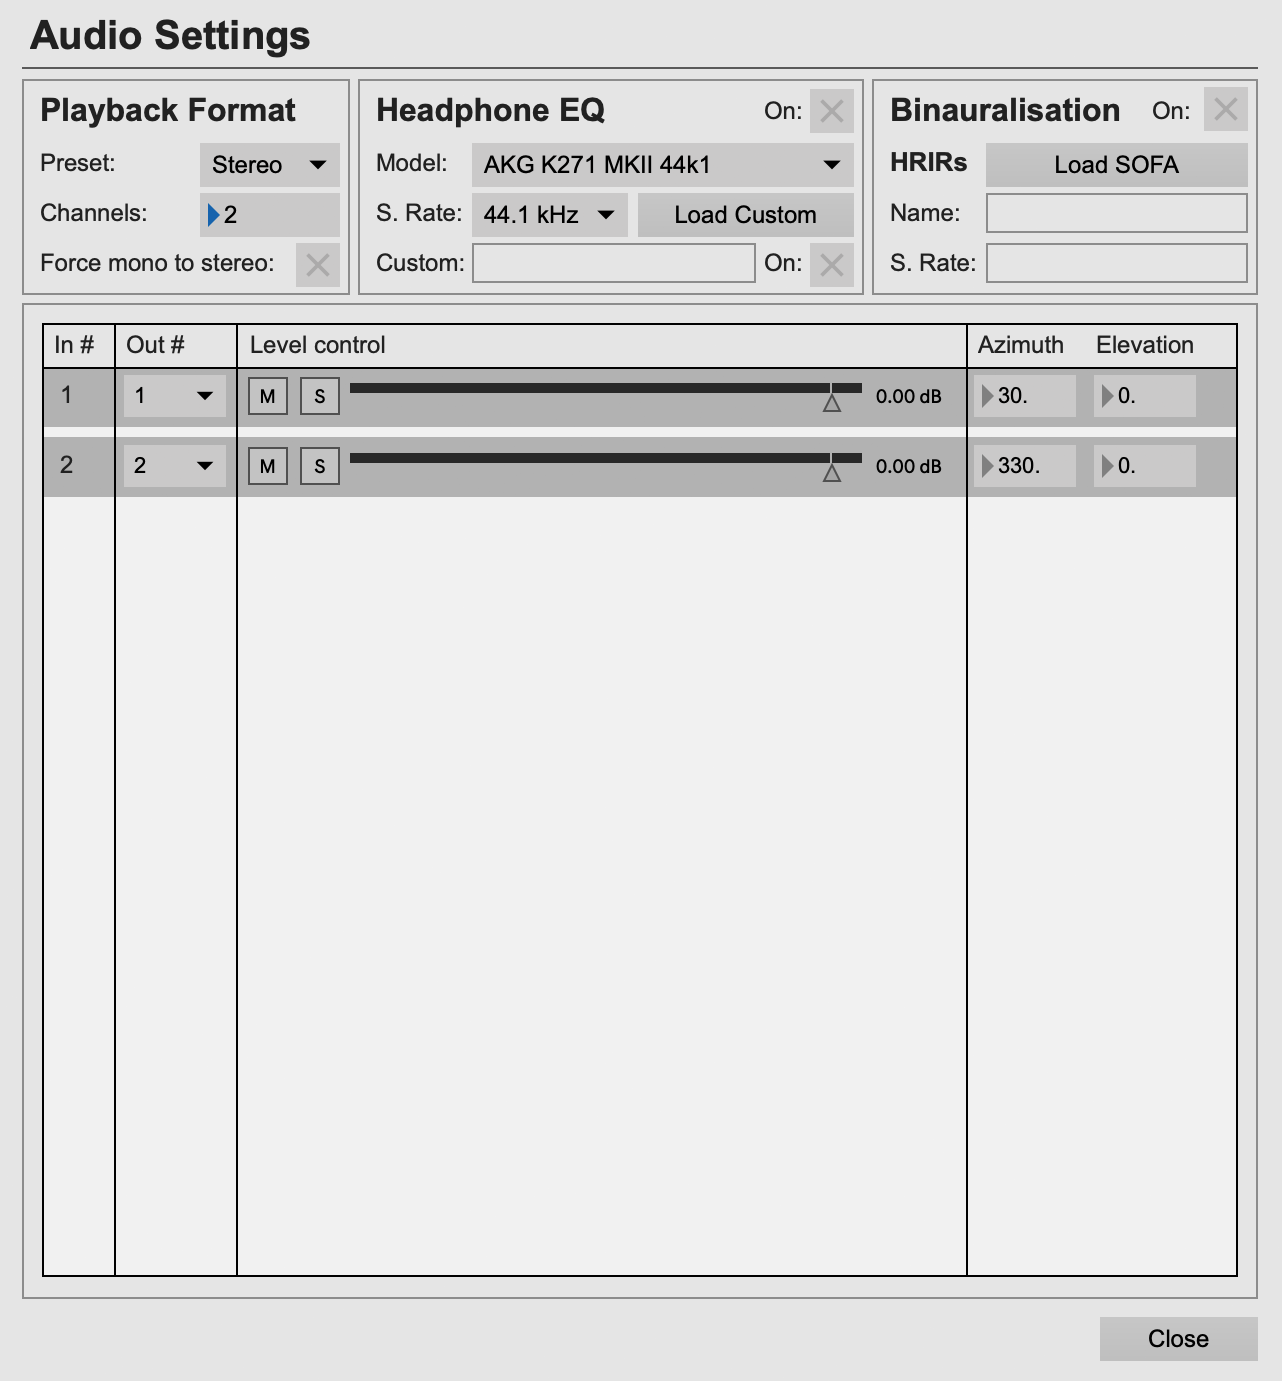
\includegraphics[width=0.7\textwidth]{./images/audioSettings_main.png}
	\caption{Audio settings screen.}
	\label{audioSettings::main}
\end{figure}

\noindent
The audio settings screen is split into four main parts: 'Playback Format', 'Headphone EQ', 'Binauralisation', and the channel list.

\section{Playback format}
The 'Playback Format' section allows you to define the number of output channels you will be using in you test, and is linked to the channel list. Here is a summary of the controls in this section:
\begin{description}
	\item[Preset] Set the channel list and 'Binauralistion' virtual speaker layout to one of the built-in configurations, e.g. 2.0, 5.0, 9.0 etc.
	\item[Channels] Sets the number of channels that will be used in the audio stream.
	\item[Force mono to stereo] Copies channel 1 to channel 2 for when you are using a mono stimuli but wish to use 2 a channel stereo loudspeaker setup or headphones.
\end{description}

\section{Headphone equalisation}
If you are using headphones for your test, it is sometimes desirable to reduce or \emph{cancel out} the effect of the headphone's own frequency response. The 'Headphone EQ' section allows you to apply headphone equalisation, either by using a matching, built-in, EQ filter, or by loading your own filter. The following is a summary of the controls in this section:
\begin{description}
	\item[Model] Selects which of the built-in headphone equalisation filter you want to use.
	\item[Load Custom] Allows you to load your own measured, headphone EQ, inverse filter.
	\item[Custom] This text box displays the filename of your custom filter. 
\end{description}
\noindent
The equalisation is enabled by toggling the top 'On' switch, whilst the custom filter is used in place of the built-in filter by toggling the 'On' switch next to the 'Custom' filename box.
\linebreak\linebreak
\noindent
\textit{\textbf{Warning:} The current version of HULTI-GEN does not feature any form of resampling of headphone EQ filters. Therefore, it is crucial that you the sample-rate of your chosen filter matches the sample-rate of Max or vice-versa.}

\section{Binauralisation}
Finally, the 'Binauralisation' section allows you to convert each audio channel into a virtual loudspeaker. The position of this virtual loudspeaker is set by the 'Azimuth' and 'Elevation' number boxes in the channel list. This process requires a Head Related Impulse Response (HRIR) database in the form of a SOFA file. These files are available from the internet. The following list describes the controls for this section:
\begin{description}
	\item[Load SOFA] Opens a dialog that lets you browse for and load a SOFA file. Binauralisation is only possible once a SOFA file has been loaded.
	\item[Name] Displays the filename of the currently loaded SOFA file.
	\item[S. Rate] Abbreviation of sample-rate, displays the sample-rate of the SOFA file.
\end{description}

\noindent
\textit{\textbf{Warning:} The current version of HULTI-GEN does not feature any form of resampling of HRIRs. Therefore, it is crucial that you the sample-rate of your chosen SOFA file matches the sample-rate of Max or vice-versa.}